\section{Participatory Design Findings}
The user group during the participatory design was a team of six third year students from The Animation Workshop in Viborg, Denmark who were developing a 3D point-and-click adventure game \cite{adventure_genre}.  The team consists of students from two different educations of the school; Character Animation and Computer Graphics Arts \cite{taw_degrees}. The students will from here on be referred to as the artists.
All the artists are familiar with making animation films with Autodesk Maya, however it is the first time they are making a video game. At the start of the project, the artists received an introductory course to the Unity game engine.

To create a tool that takes the artists' current skills and experience into consideration, thereby easing their learning curve, we used techniques from participatory design \cite{part_design}.

\subsection{Activities}
%\textbf{Write this with an active voice}
Four different activities using a combination of participatory design techniques were conducted with four artists from the team who had an interest in working with the camera tool. All activities were combined with open interviews as well as video recorded for further analysis and took 15-30 minutes per person.

The first activity, was an observation \cite{part_design} of the artists working in Maya and Unity. The artists were asked to think-aloud \cite{part_design} while performing simple tasks relevant to camera work in Maya and Unity. The purpose of this activity was to gain firsthand experience with the artists' current work practices in Maya as well as an understanding of how familiar they were with Unity.

Second, the artists were asked to list and sketch the features that they would like to see the most in the camera tool. This activity took inspiration from the Freehand Drawing technique \cite{part_design}. The purpose of the activity was to get a foundation for which tasks the artists wanted to be able to do with the tool.

After sketching, the artists were asked to visualize the interface of the camera tool with a set of pre-made buttons and windows out of paper based on Unity's interface (see Figure \ref{fig:collage}). The activity took inspiration from the Collage technique \cite{part_design} and its purpose was to get a foundation for the interface design.

\begin{figure}[htbp]
\centering
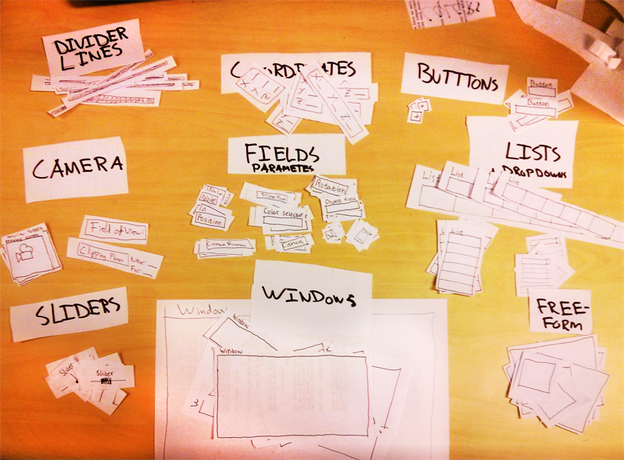
\includegraphics[width=0.3\textwidth]{Pics/labels}
\caption{The collage activity. The camera settings and general interface were made out of paper.}
\label{fig:collage}
\end{figure}

The final activity was made after the first design iteration of the tool. At this point, the features that were assessed as most important for the artists had been implemented, however it was still necessary to receive input from the artists. Using the same techniques as in the initial observation, we had the artists perform simple tasks in Unity with the camera tool. From this, it was possible to see which changes should be made to the tool, especially regarding the interface.

\subsection{Findings} \label{findings}
From the previously mentioned activities, we found that the artists in general want features as well as an interface in the camera tool that are similar to those found in Maya's interface.

The artists deemed it essential that the camera tool should give the artists the freedom to frame the scene as they want, in order to focus on different elements in the scene.

An important feature the artists use heavily in Maya when animating a camera in a scene, is keyframing, i.e. the artists place points on a timeline, and at each point adjust the camera according to how they want to frame the scene.

%There are multiple ways to adjust the camera in Maya. It can be done by manually adjusting the X, Y and Z position and rotation of the camera; moving it by dragging a handle tool; deciding the forward direction of the camera by using the \textit{Camera Aim} feature \cite{maya_camAim} or, alternatively, by using the the \textit{Look Through Selected} feature \cite{maya_lookThrough}. 

During the initial observations, it was clear that many of the artists preferred the \textit{Look Through Selected} feature in Maya \cite{maya_lookThrough}.

When the artists needed control over how the camera should interpolate between keyframes, they used Maya's \textit{Graph Editor} \cite{maya_graph}, which allowed them to adjust the interpolation for all camera settings using \textit{animation curves} \cite{maya_graph}. The artists often adjusted multiple curves at the same time and in the same window.
%\textbf{(Argument for discussion chapter that we didn't include this)}

We also observed that all of the artists work with two monitors and that they often spread Maya's interface out across both monitors to take better advantage of the space. They did this by creating separate windows for certain features. 

A common request from all of the artists was the ability to quickly preview their changes. Instead of having to start the game and navigate the player character to a specific framing, the artists wanted to quickly jump to a specific framing to test out how it feels and looks.

Finally, we observed that the artists found Unity's \textit{Flythrough Mode} \cite{unity_flyMode}) particularly useful. This feature lets the player fly around with the scene camera as if they were playing a first-person game.

%It was discovered that none of the artists knew how to use a standard Unity feature that lets the player fly around with the scene camera as if they were playing a first-person game ("Flythrough Mode", \cite{unity_flyMode}). The artist were excited about the discovery of this feature. One artist perceived the standard way of moving around in Unity as confusing, while another stated that the way of moving the camera is exactly like in Maya. After testing this ourselves, we concluded that the movement controls in Maya and Unity are indeed very similar (except for the "Flythrough Mode"), which means that the artists should ideally be comfortable with navigating in either of the applications.


%A keyframe is an event and/or change in one or more parameters over time. Each keyframe corresponds to a point in time, meaning that when the animation reaches this point in time, the values of this keyframe are dominant. Usually this means that in between keyframes some interpolation is happening. This interpolation is per default linear, but can be manipulated in a graph editor. Anything that can be represented by numbers can be manipulated through keyframes.

%In Maya, there are multiple ways to accomplish the same thing. An example of this is how to adjust a camera in the scene. This can be done by manually adjusting the X, Y and Z position and rotation of the camera; moving it by dragging a handle tool; or, alternatively, by using the the \textit{Look Through Selected} feature \cite{maya_lookThrough}. During the initial observations, it was clear that many of the artists at The Animation Workshop preferred the latter. This concept was translated directly into the camera tool. Using the \textit{be the camera} feature (see Figure \ref{fig:beTheCam}), the artists can place their camera by navigating the scene in Unity with the \textit{Flythrough mode} \cite{unity_flyMode}.

%It was discovered that none of the artists knew how to use a standard Unity feature that lets the player fly around with the scene camera as if they were playing a first-person game ("Flythrough Mode", \cite{unity_flyMode}). The artist were excited about the discovery of this feature. One artist perceived the standard way of moving around in Unity as confusing, while another stated that the way of moving the camera is exactly like in Maya. After testing this ourselves, we concluded that the movement controls in Maya and Unity are indeed very similar (except for the "Flythrough Mode"), which means that the artists should ideally be comfortable with navigating in either of the applications.

%\subsection{Conclusion}
%Through the participatory design exercises, we found that the artists were very familiar with Autodesk Maya \cite{MayaSource}. To ease the learning curve, we decided to design the tool with the overall structure of Maya in mind. This doesn't mean that the tool should directly copy how Maya looks and works, but that, when designing the camera tool, we should keep their established mental models \cite{mentalModels} in mind. Since the artists have been working with Maya and other 3D modelling software, they have a certain understanding and expectation of the animation process. As a designer, you create conceptual models for the system. Therefore, it's important to be aware of the users' pre-existing mental models. Another key finding was the fact that most of the artists were working with two computer monitors. This enables them to have the main interface on one monitor, while the other can show secondary windows such as graph editors or an additional preview window showing the camera's point of view.